\chapter{RDE prototype infrastructure}\label{ch:rde-prototype-infrastructure}
In this chapter we will explain the infrastructure that we have developed for the FileSender RDE prototype.
We also refer to the technical documentation in the repositories of the components for more information on the individual parts.

\section{Overview}\label{sec:rde-prototype-infrastructure-overview}
The infrastructure for RDE consists of the following components:
\begin{itemize}
    \item A \emph{FileSender} instance, which is the regular filesender application server that is hosted by SURF and receives the encrypted files and allows recipients to download them.
    \item An \emph{RDE key server} that is responsible for collecting enrollment data for users, verifying their email addresses and making them available for querying by senders.
    \item An \emph{RDE client} application that is able to interact with a user's passport via NFC during enrollment and decryption (key retrieval).
    \item The RDE browser client of the sender, which will run in the browser of the sender and will be used to generate the RDE keys (the secret key and decryption parameters).
    This component will be included in the FileSender web application, but will run in the browser and not on the server.
    \item The RDE browser client of the recipient, which will run in the browser of the recipient and will be used to receive the retrieved key from the RDE client app and decrypt the file.
    This component will also be included in the FileSender web application, but will run in the browser and not on the server.
    \item A simple \emph{proxy server} that will enable communication between the RDE client app and the RDE browser client of the recipient.
\end{itemize}

We first describe a general infrastructure for RDE in arbitrary applications.
Then we describe the integration in FileSender in particular.
We also give some considerations specific to the SURFfilesender application.

The general infrastructure is presented in Figure~\ref{fig:rde-prototype-infrastructure-overview}.
\begin{figure}
    \centering
    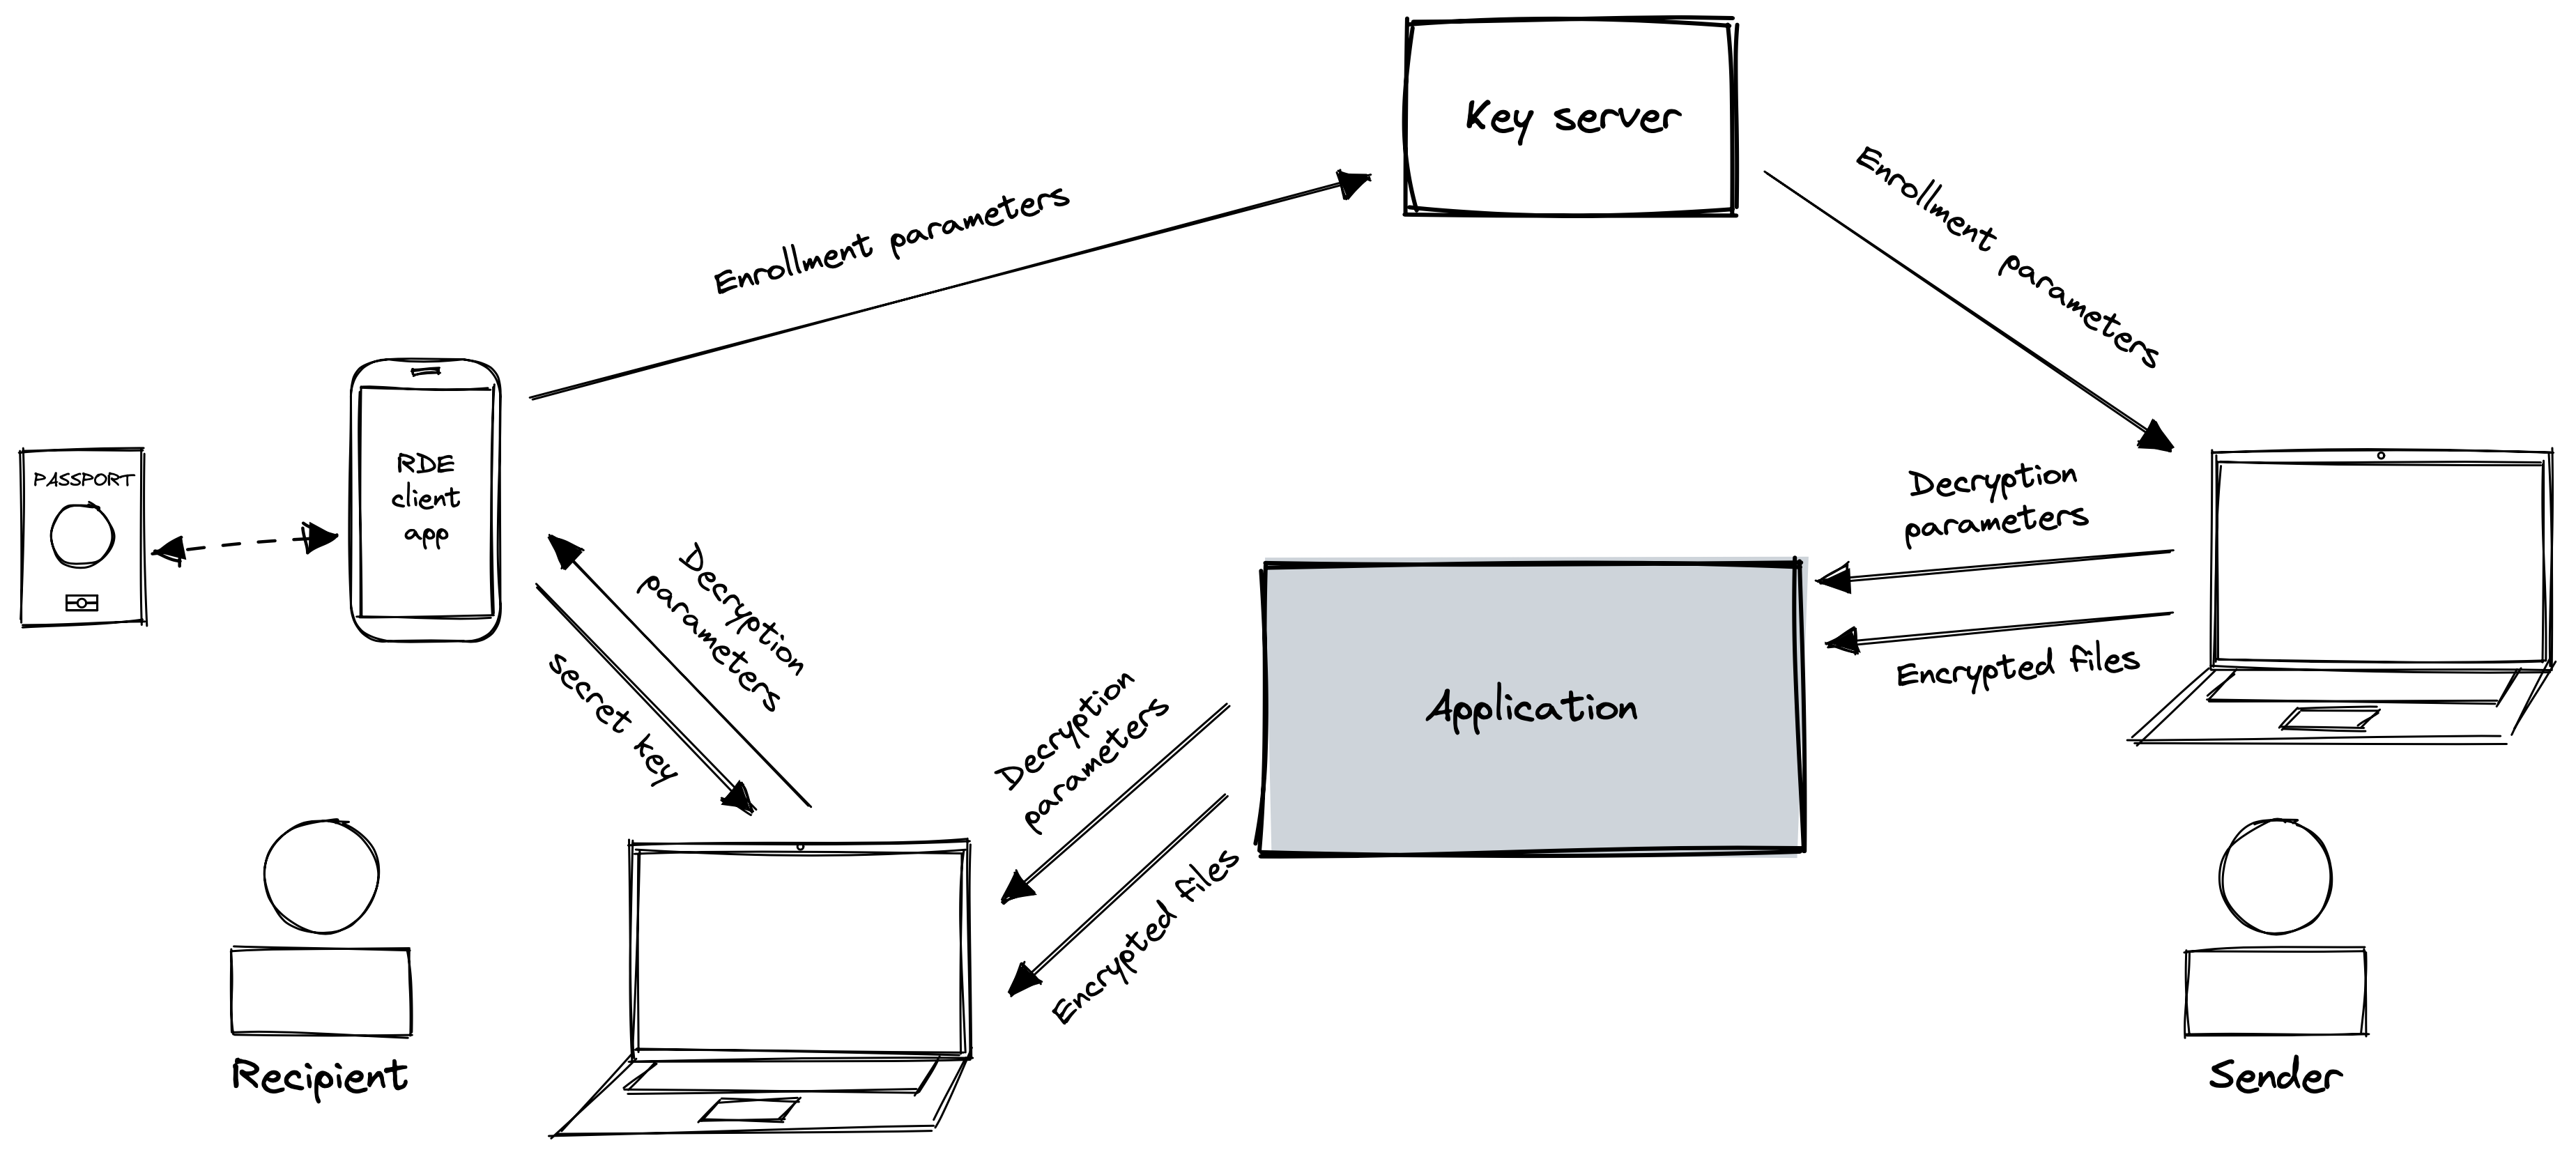
\includegraphics[width=\textwidth]{imgs/RDE infra overview}
    \caption{Overview of the RDE prototype infrastructure.
    A more detailed figure for each phase of RDE is included in Figure~\ref{fig:rde-detail}.}
    \label{fig:rde-prototype-infrastructure-overview}
\end{figure}

\begin{figure}
    \centering
    \begin{subfigure}[b]{0.5\textwidth}
        \centering
        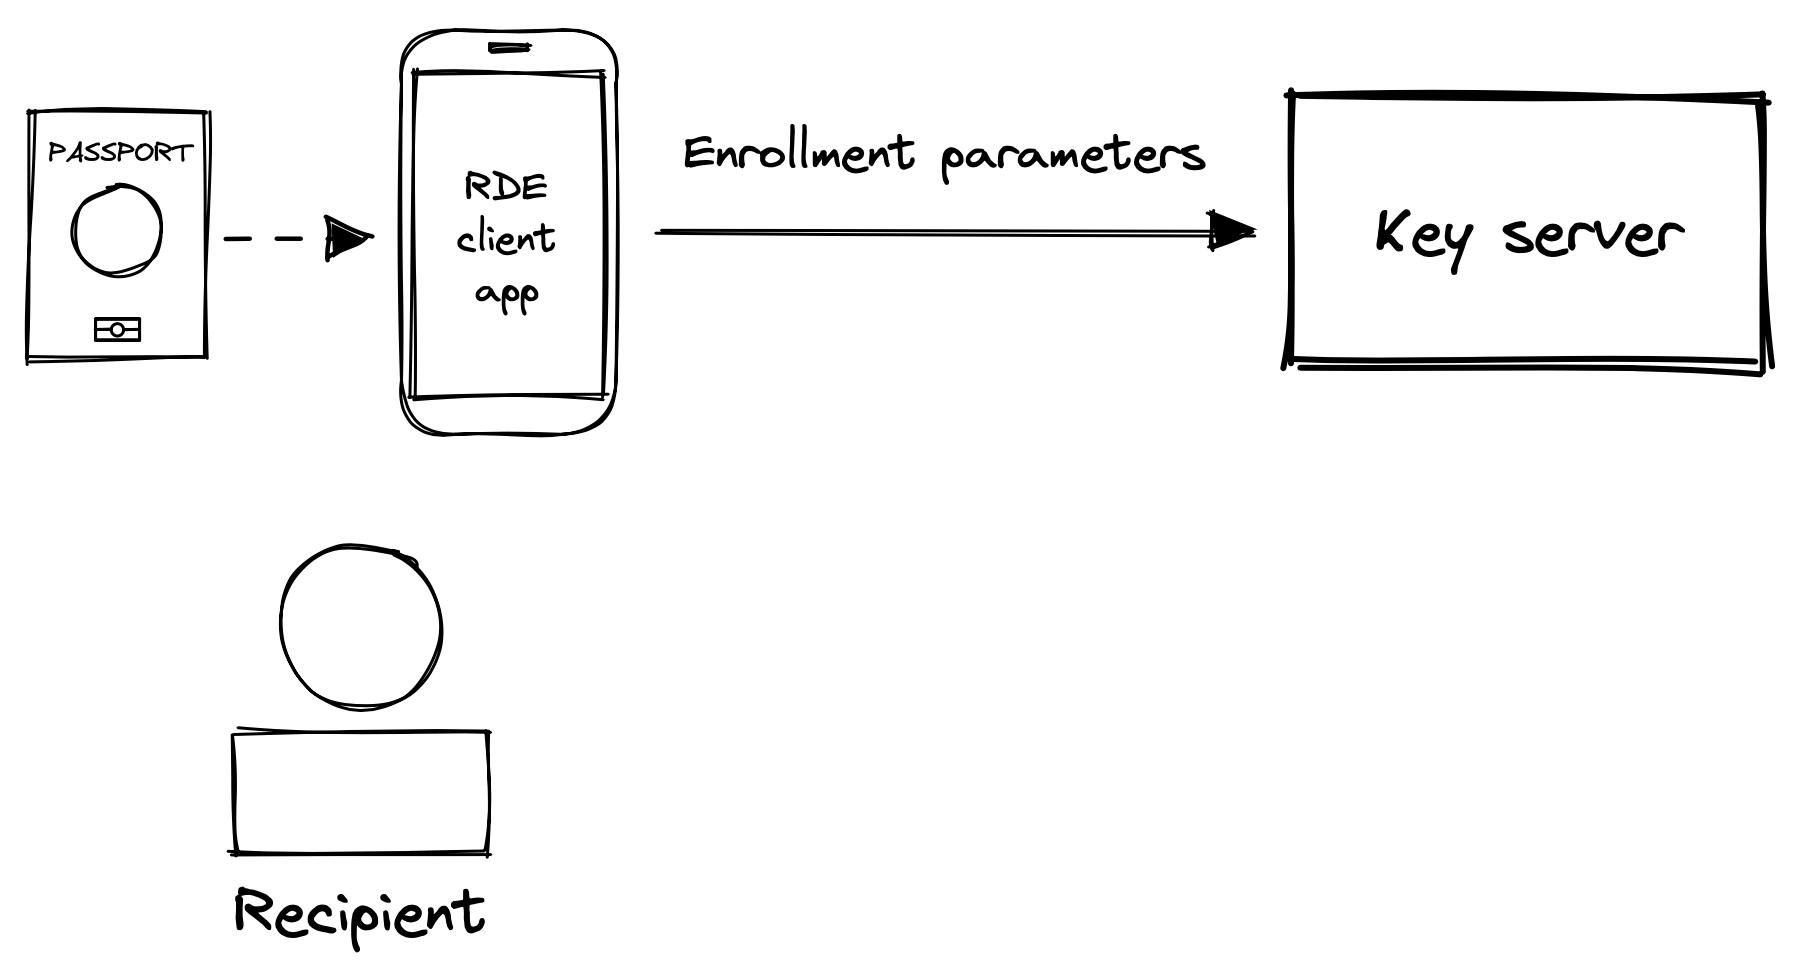
\includegraphics[width=\textwidth]{imgs/RDE enrollment detail}
        \caption{Enrollment}
        \label{fig:rde-enrollment-detail}
    \end{subfigure}\\
    \vspace{1cm}
    \begin{subfigure}[b]{0.8\textwidth}
        \centering
        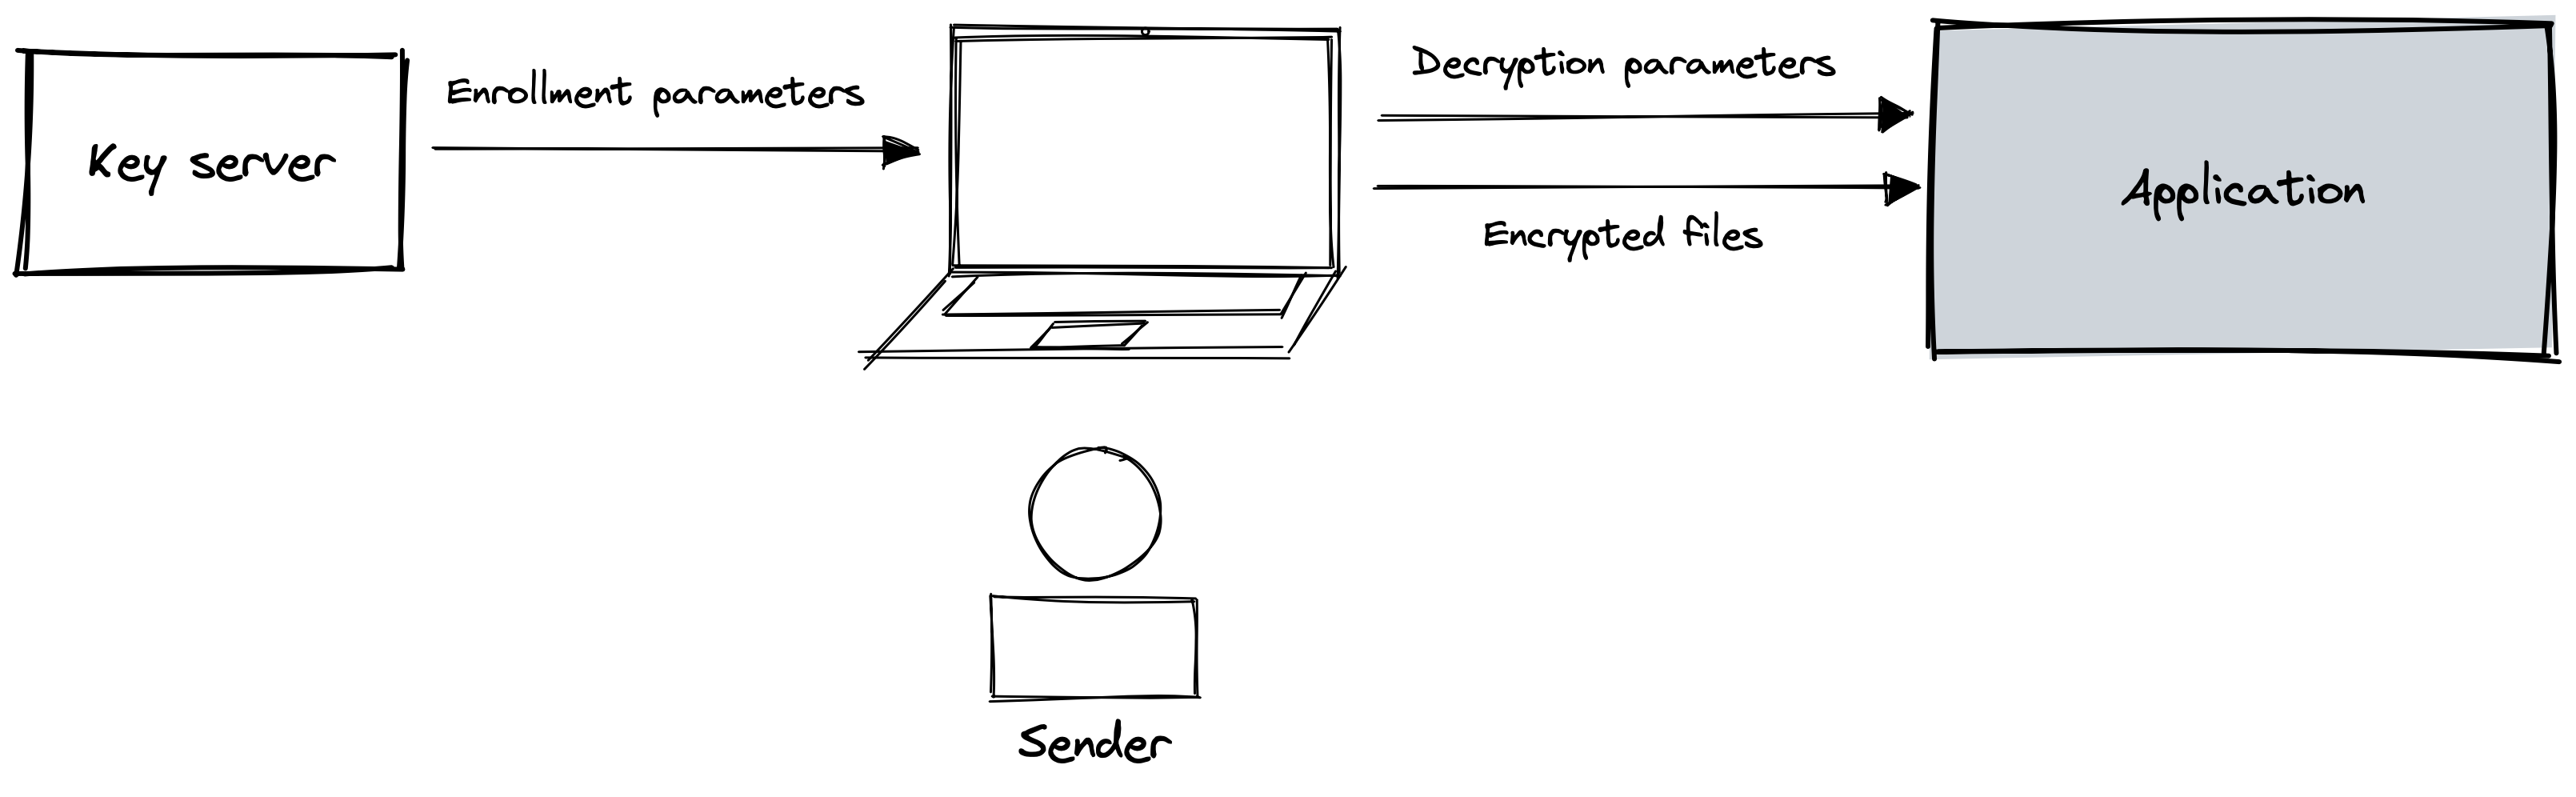
\includegraphics[width=\textwidth]{imgs/RDE keygen detail}
        \caption{Key generation}
        \label{fig:rde-keygen-detail}
    \end{subfigure}\\
    \vspace{1cm}
    \begin{subfigure}[b]{0.8\textwidth}
        \centering
        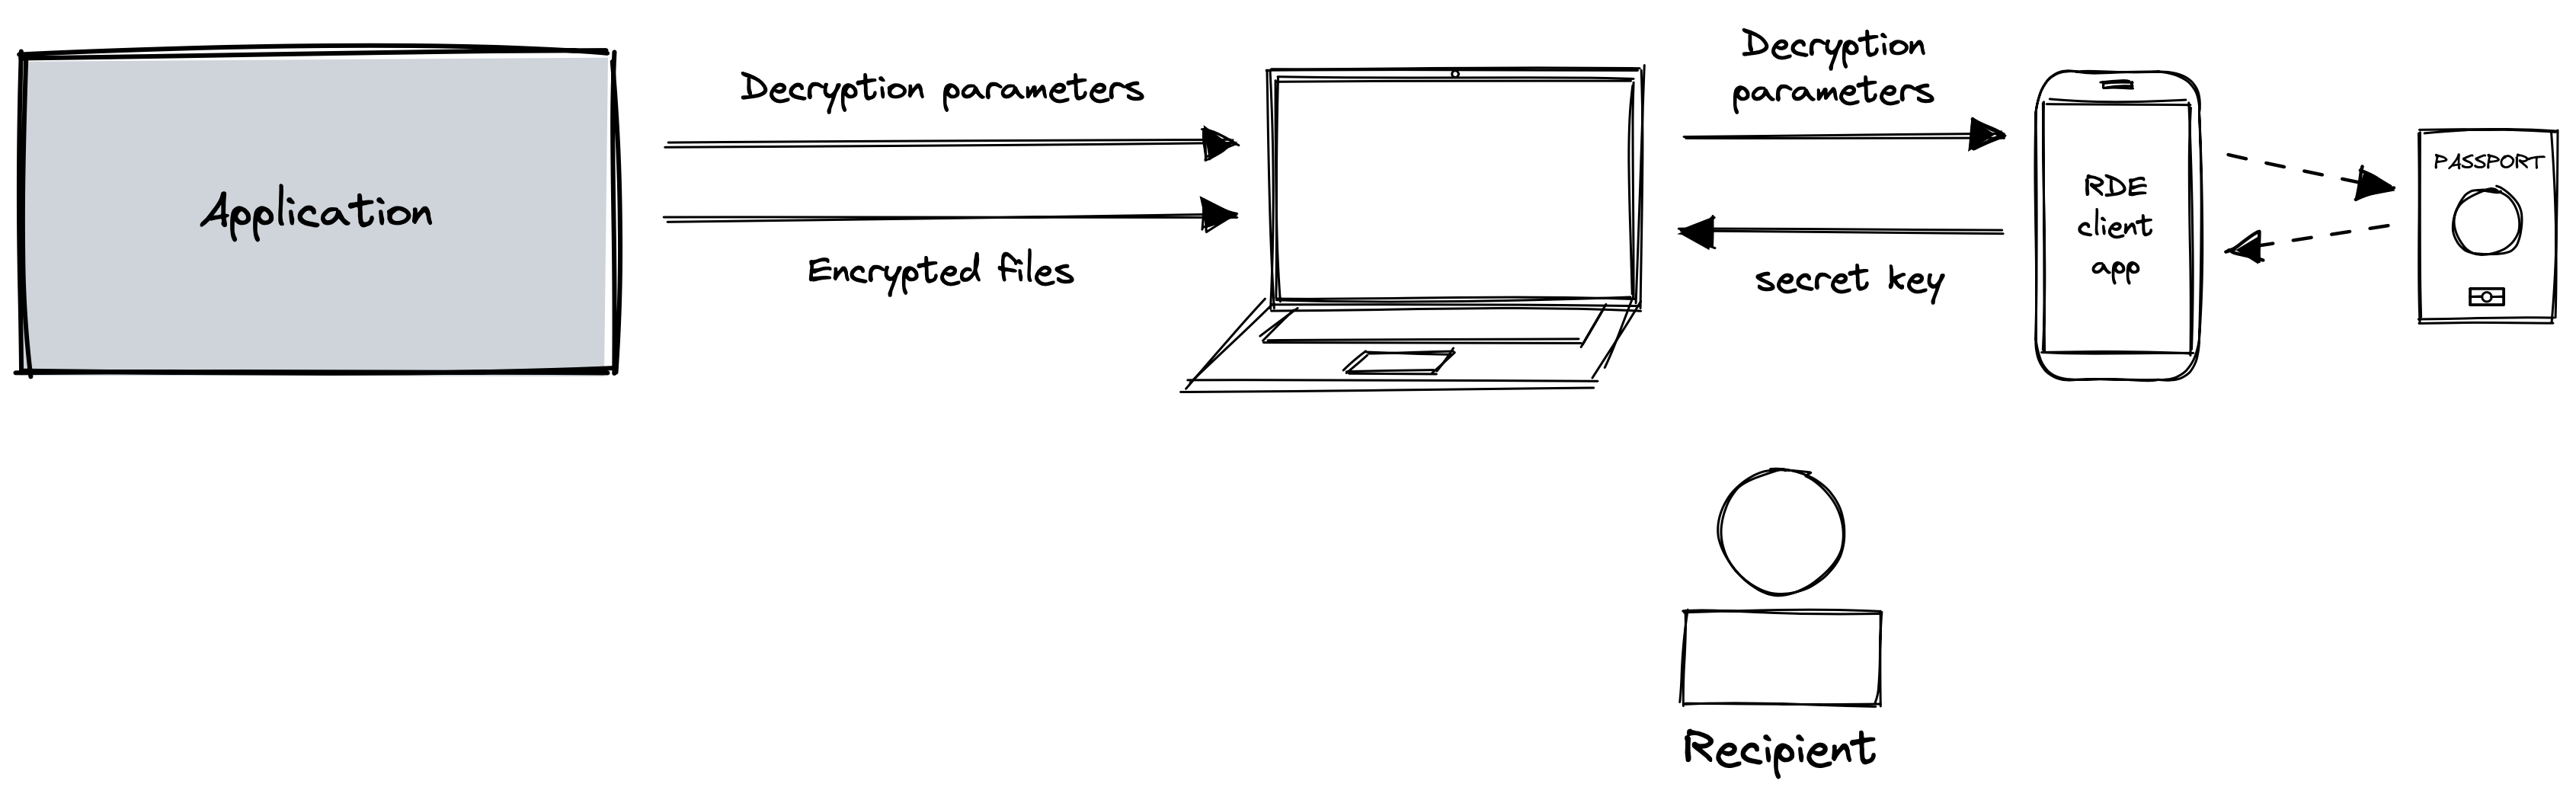
\includegraphics[width=\textwidth]{imgs/RDE decryption detail}
        \caption{Decryption}
        \label{fig:rde-decryption-detail}
    \end{subfigure}
    \caption{Interaction in the RDE prototype infrastructure in different phases.}
    \label{fig:rde-detail}
\end{figure}

\subsection{Notes on our implementation}\label{subsec:infrastructure-overview-notes-on-our-implementation}
For the prototype, we have implemented components that can be grouped into 3 categories:

First, there are the core RDE components that enable the enrollment, key generation and decryption (key retrieval) steps of the basic RDE scheme.
These consist of a Java library written in Kotlin for the interaction with the e-passport, and a TypeScript library for the key generation and passport emulation.
The latter is written in TypeScript, as it is intended to be used in a browser environment by the end user.
Their implementation is also independent of the actual application in FileSender, and can be used for other applications or infrastructures for RDE as well.

Second, there is a category of infrastructure components that are needed to make the RDE prototype work.
These are the RDE key server that stores enrollment data, the client app that enables enrollment en decryption and that uses the aforementioned library, and a simple proxy server that allows communication between the client app and the browser client of the recipient.
These components are minimal implementations that are sufficient for the prototype, but are not intended to be used in production in their current form, as they are not secure and do not have all the features that would be needed for a production system.
These components are still independent to the FileSender application, and can be used for other applications as well that use the same infrastructure.

Finally, there is the integration of RDE in the FileSender application itself.
Here, minimal changes have been made to the FileSender application to enable the RDE functionality.

\section{Core components}\label{sec:core-components}
The core components of the RDE prototype are the Java (Kotlin) library and TypeScript library for key generation that provide the cryptographic functionality for the RDE scheme.
This includes the interaction with the e-passport for enrollment, the key generation and the decryption (key retrieval) steps.
The Java library basically forms a wrapper around the JMRTD library\footnote{\url{https://jmrtd.org}} for interaction with an e-passport and uses the BouncyCastle library\footnote{\url{https://www.bouncycastle.org}} for the cryptographic operations.
The TypeScript library is intended to be used in a browser environment by the end user and does not implement any steps that require interaction with the passport.
In the future, however, it could be interesting to implement this in the browser as well, as this would allow for a more seamless user experience.
This would require hardware support for NFC in the browser.

\subsection{Data classes}\label{subsec:data-classes}
There are several data classes that are used to store data / messages within the RDE protocol.
For our prototype, we have chosen for simple JSON objects, as they are easy to work with and can be easily converted to and from byte arrays.

\subsubsection{\textsf{RDEEnrollmentParameters}}\label{subsubsec:rdeenrollmentparameters}
The \textsf{RDEEnrollmentParameters} class is used to store the enrollment parameters for an e-passport.
This class includes the following fields:
\begin{itemize}
    \item \textsf{documentName}: a user-chosen name for the e-passport (mnemonic name), which is used to identify the e-passport towards the user (for example ``\textsf{My passport (******ABC)}'', showing the last 3 digits of the 9-digit document number).
    \item \textsf{rdeDGId}: the data group ID of the data group to read for RDE (usually 14).
    \item \textsf{rdeDGLength}: the number of bytes to read for RDE (usually 223, the maximum plaintext size for which the ciphertext fits in a single APDU).
    \item \textsf{rdeDGContent}: the plaintext contents of the data group to read for RDE (usually the first 223 bytes of the data group, or the full data group if we do include the EFsod in the enrollment parameters), as a hexadecimal string.
    \item \textsf{caOID}: the OID of the CA protocol supported by the e-passport.
    \item \textsf{piccPublicKey}: the public key of the CA protocol supported by the e-passport, as a hexadecimal string ASN.1 X9.62 TLV (Tag-Length-Value)-encoded public key (according to ICAO specification, X9.42 for RSA based DH and TR-03111 for ECDH~\cite{icao9303securitymechanisms}).
    \item \textsf{securityData}: the contents of EFsod, as a hexadecimal string, or null if the EFsod is not included in the enrollment parameters.
    \item \textsf{mrzData}: the contents of DG1, as a hexadecimal string, or null if the MRZ is not included in the enrollment parameters.
    \item \textsf{facialImageData}: the contents of DG2, as a hexadecimal string, or null if no facial image is included in the enrollment parameters.
\end{itemize}

\subsubsection{\textsf{RDEKey}}\label{subsubsec:rdekey}
The \textsf{RDEKey} class is used to store a generated RDE key, as generated by a sender.
It consists of the secret key (byte array) that can be used to encrypt an decrypt messages, and the decryption parameters that can be made public and that are used together with the e-passport to retrieve the secret key.

\subsubsection{\textsf{RDEDecryptionParameters}}\label{subsubsec:rde-decryption-parameters}
The \textsf{RDEDecryptionParameters} class is used to store the decryption parameters that are used to retrieve the secret key.
It consists of the ephemeral public key chosen by the sender and the protected command that should be sent to the e-passport to retrieve the secret key.
The public key is a X.509 hexadecimal encoded ASN.1 DER string according to ICAO specification (X9.42 for RSA-based DH and TR-03111 for ECDH~\cite{icao9303securitymechanisms}), and the protected command is encoded as a hexadecimal string.
Additionally, the OID\footnote{Object identifier, a globally standardized identifier for, among others, cipher suites.} of the CA algorithm is stored, as having this information saves us a step in the decryption process.

\subsection{Enrollment}\label{subsec:enrollment}
Enrollment is only included in the Java (Kotlin) library, as it requires interaction with the e-passport.
During enrollment, first, the security info is read from the e-passport in order to determine if the e-passport supports PACE or if we should fallback to BAC for our first level of secure messaging.
If PACE is supported, we use PACE to authenticate to the e-passport, otherwise we use BAC.

After authentication, we read the data group that is chosen to be used for RDE.
Usually, you want this to be data group 14, as this group is usually of sufficient size and does not contain privacy sensitive data, but other data groups that can be read without Terminal Authentication are also supported.
If enrollment with MRZ data is chosen, we also read data group 1, which contains the MRZ data.
If enrollment with facial image data is chosen, we also read data group 2, which contains the facial image data.
Finally, we also read the EFsod, which contains the security data of the e-passport.

Then, we perform passive authentication with the information from the EFsod.
Note that in the current implementation, we do not check the certificate chain of the EFsod, as this is not necessary for the prototype and would require us to include a certificate store with trusted certificates.
In the future, this should be added to the implementation.

For enrollment, apart from the data group to use for RDE, users can also choose the number of bytes to read from that data group, $n$ or \textsc{rdeDGLength}.
This usually is 223, as this is the maximum plaintext size for which the ciphertext fits in a single APDU, but can also be less if the user agrees with weaker security.
Note that the data group must be large enough to actually read the number of bytes chosen by the user.
Especially data group 1 is too small to read 223 bytes, so we recommend using data group 14 for enrollment.

If enrollment with security data is chose, we include the EFsod in the enrollment parameters, together with the full contents of the RDE data group.
If enrollment with MRZ data is chosen, we also include the MRZ data in the enrollment parameters, and similarly for facial image data.
If no security data is included, we only include the first $n$ bytes of the RDE data group, as this is the maximum plaintext size for which the ciphertext fits in a single APDU and we thus do not need more data.
If we do include security data, we must include the full RDE data group, as the hash of the RDE data group otherwise will not verify with the EFsod.

We also include the OID of the CA protocol supported by the document, as this is needed to determine the public key format, cipher algorithms and key length during key generation.

Finally, the enrollment parameters include a document name, which functions as a mnemonic name to identify the document towards the user (in case the user has multiple documents enrolled).

\subsection{Key generation}\label{subsec:key-generation}
Key generation is included in the TypeScript library, as it does not require interaction with the passport and is expected to run in the browser of a sender.
For completeness, however, we also include key generation in the Java (Kotlin) library, as it is useful for testing purposes and could potentially be useful for other applications when a server wants to encrypt messages for a user.
However, verification of the enrollment parameters is not yet implemented in the Java (Kotlin) library.
Only the TypeScript library currently implements verification of the enrollment parameters.

The key generation takes the enrollment parameters as input, and generates a secret key and decryption parameters.
This is done by first generating a ephemeral key pair for the offline CA (EC)DH key agreement, compatible with the CA protocol supported by the e-passport.
We then compute the shared secret using the ephemeral private key and the public key of the e-passport.
From the shared secret, we derive the KMAC and KENC keys according to the ICAO specification for the supported CA protocol.

The most significant step is then to emulate the e-passport response to a READ BINARY command for the RDE data group, using KENC to encrypt the data group and KMAC to compute the MAC.
This results in the emulated ciphertext, which is then used to generate the secret message key by simply taking the SHA-256 hash of the ciphertext.
We also generate the encrypted READ BINARY command with KENC and KMAC and store this, together with the ephemeral public key, in the decryption parameters.

The main difference between the key generation in the TypeScript and Java (Kotlin) library is that the Java (Kotlin) library uses the Bouncy Castle library for all cryptographic operations and implementations from JMRTD, while for the TypeScript library these are not available.
The TypeScript library also cannot use the WebCrypto API for these steeps, as it does not support all algorithms and curves that are used in the ICAO specifications.
We therefore use custom crypto libraries for emulating the passport response and generating the protected command.
For more details, we refer to our source code.

\subsubsection{Verification of enrollment parameters}\label{subsubsec:verification-of-enrollment-parameters}
Before generating the secret key, we can verify the enrollment parameters to authenticate the document holder as described in Chapter~\ref{ch:rde-with-document-holder-authentication}.
This, naturally, is only possible if the enrollment parameters include security data.

First, the hashes on the chosen RDE data group, and optionally the MRZ data and facial image data, are verified against the hashes in the EFsod.
Then, the hash on the full EFsod is verified, followed by the signature on this data.
Finally, the certificate chain of the EF.SOD is verified against a trusted certificate store.

Any user can choose their own trusted certificates.
This means that a user can determine themselves which certificates from which issuing states they trust.
For the prototype, we use 13 certificates from the Dutch government Country Signing Certificate Authority (CSCA)\footnote{\url{https://www.npkd.nl}}.
Parsing a `Masterlist file' that contains a list of certificates from multiple CSCAs not yet implemented.
Certificates need to be provided individually in PEM format.
Also CRL's (Certificate Revocation Lists) are not yet implemented.

\subsection{Decryption (key retrieval)}\label{subsec:decryption-key-retrieval}
Decryption is only included in the Java (Kotlin) library, as it requires interaction with the e-passport.
During decryption, similar to enrollment, first, the security data of the e-passport is read from the e-passport and either PACE or BAC is used to authenticate to the e-passport.
Then, we perform Chip Authentication with the ephemeral public key from the decryption parameters.
The e-passport will now further communicate with the reader using the shared secret with the sender who created the decryption parameters.
We then send the protected command from the decryption parameters to the e-passport, which results in ciphertext contents of the RDE data group.

We derive the secret message key from the ciphertext by simply taking the SHA-256 hash of the ciphertext.

We reiterate that the ciphertext that forms the basis for the secret key, is sent in the clear from the e-passport to the reader (that computes the SHA-256 hash).

\subsection{Cryptography implementations}\label{subsec:cryptography-implementations}
As mentioned earlier, cryptographic operations in the Kotlin library use JMRTD and BouncyCastle.
This is the obvious choice, as JMRTD is a solid library that implements communication with e-passports, and already uses BouncyCastle.

For the TypeScript libraries, the preferred solution would be to use the WebCrypto API, as it is the most secure and most efficient implementation.
The WebCrypto API, however, does not support all cryptographic operations that are required for emulating a passport, such as AES-CMAC or elliptic curve cryptography with brainpool curves.
That is why we have chose to use the following cryptographic libraries for emulating e-passport commands and responses:

TODO

\section{Infrastructure components}\label{sec:infrastructure-components}
The infrastructure components of the RDE prototype are the key server, the proxy server and the reader app.
They function as a minimal implementation of the RDE prototype and work independently of the FileSender application (or any other application for that matter).

\subsection{Key server}\label{subsec:key-server}
The key server in its most simple form is a simple REST API that stores the enrollment data and allows users to query it.
Our implementation is written in Python and uses the Django web framework.
Users can register and log in to the key server using SURFconext, which is a federated identity provider.
Via SURFconext, the key server receives the user's email address which will be used to link the enrollment data to.
Users can then use the reader app to enroll their e-passport and push the enrollment data to the key server.

\subsubsection{Querying the key server}\label{subsubsec:querying-the-key-server}
The key server provides a REST API for querying the enrollment data based on the user's email address.
The key server will then return the enrollment data for the user, if it exists.

It is important to note that by storing all enrollment data on the key server, this key server contains a lot of privacy sensitive information.
If users choose to use document holder authentication during enrollment, the key server might contain the MRZ data and facial image data of the user.
We should thus be careful with making the key server available to the public.
Probably, we should only allow certain authenticated users to query the key server.
This is not implemented in the prototype and is topic for further discussion.

\subsubsection{Key server security}\label{subsubsec:key-server-security}
There are a number of security assumptions that we make about the key server.
\begin{itemize}
    \item For senders, we do trust the key server to return the correct enrollment data for a user's email address.
    \item For senders, we do \emph{not} need trust the key server to not modify the enrollment data if the data includes document holder authentication.
    Senders can verify the enrollment data themselves.
    \item For recipients enrolling at the key server, we do trust the key server to handle the enrollment data securely with respect to the user's privacy.
\end{itemize}
In this sense, the security assumptions towards the RDE key server are similar to those of other key servers, such as for PGP.

\subsubsection{Notes on our implementation}\label{subsubsec:keyserver-notes-on-our-implementation}
The implementation of the key server for our prototype is very minimal.
The API for querying the key server is very simple and does not include any authentication for querying users or rate limiting.
The key server also does not verify the enrollment data upon receiving it.
Finally, it provides no way to delete enrollment data.
The process of scanning a QR code for enrolling e-passports is an easy implementation, but not very user friendly and not very secure.
For a production system, these features should be implemented.

\subsubsection{SURFconext and eduID}\label{subsubsec:surfconext-and-eduid}
One approach for implementing a production key server at SURF is to integrate it within eduID, another service SURF offers.
eduID can be considered as an universal identity service that contains different attributes about a user.
In contrast to regular SURFconext, where attributes are provided by institutions, eduID attributes are stored by SURF itself.
This means that eduID can be used to store attributes that are not provided by institutions, such as the RDE enrollment parameters.

A user's RDE `public key' (enrollment parameters) could thus be stored as attributes in eduID.
This would, however, still require a key server to be implemented for querying the enrollment parameters for users.
It is thus questionable whether this would be a good approach for implementing an RDE public key server at SURF, at least not necessarily for filesender applications, where senders need to query for enrollment parameters of other users.
Only in situations where the sender is a server, encrypting information for the user itself, would this approach be useful.

\subsection{Proxy server}\label{subsec:proxy-server}
In order to achieve true end-to-end encryption, the browser and the app need to be able to communicate with each other.
This is not easily possible, as we cannot assume that the browser and the app are on the same network (even if they are, they can probably not communicate directly).
Therefore, we have created a proxy server that acts as a middleman between the browser and the app.
The sole purpose of this server is to relay messages between the browser and the app.
It is not involved in the actual encryption process, nor should it have any security critical role.
The proxy server is implemented in Python and uses the Flask web framework.
The proxy server simply allows websockets to be opened between the browser and the app and relays messages between them.

\subsubsection{Decryption handshake protocol} \label{subsubsec:decryption-handshake-protocol}
In order to facilitate end-to-end encryption between the browser and the app, we have created a simple protocol for the decryption handshake.
The protocol is very simple and consists of the following steps:
\begin{enumerate}
    \item The browser opens a websocket connection to the proxy server on a unique URL.
    \item The browser presents a QR code to the user that contains the URL of the websocket connection.
    \item The user scans the QR code with the app.
    \item The app opens a websocket connection to the proxy server on the same URL.
    \item The app generates a ephemeral key pair and sends the public key to the browser.
    \item The browser generates a ephemeral key pair and a random IV and sends those back to the app.
    \item Both parties perform a Diffie-Hellman key exchange using the ephemeral key pairs.
    Both parties now have the same shared secret and can communicate with each other using this shared secret.
    \item The browser sends the decryption parameters to the app, encrypted with the shared secret and the IV.
    \item The app decrypts the decryption parameters and uses them to retrieve the secret key from the passport.
    \item The app sends the retrieved secret message key to the browser, encrypted with the shared secret and the IV.
\end{enumerate}

We use ECDH with the NIST P-384 curve for the Diffie-Hellman key exchange.
For further communication, we use AES-256-CBC with a 128-bit IV.
Keys are encoded as JWKs.

We expect the connections with the proxy server to use TLS (WebSocket Secure) (and strongly rely on this for security).
This means that the proxy server will not be able to read the messages sent between the browser and the app.

This protocol is implemented in a TypeScript library for decryption, and in the reader app.
Because this protocol, however, is not part of the RDE scheme itself, we do not discuss it in depth.

\subsubsection{Attacks on the proxy server}
The proxy server is a potential point of failure in our prototype infrastructure.
An active MITM attacker could intercept the ECDH key exchange and this way be able to read the secret key that is transferred from the reader app to the browser.
This can easily be achieved by authenticating the shared secret between the browser and the app by showing a message to the user that they need to confirm on both devices, or by letting the app create a simple linking code that the user needs to enter on the browser before proceeding.
For the implementation in our prototype, we have chosen to not implement such security measures, as this does not relate to the actual RDE protocol and we consider it out of scope for this prototype.
For production systems, however, we should definitely consider implementing security measures against MITM attacks.

Phishing attacks are also a potential threat, as the user might be tricked into scanning a QR code that is not generated by the browser.
This also results in the user's secret key being leaked to the attacker.
This can be solved, too, by showing a message to the user that they need to confirm on both devices.
We have not implemented this in our prototype either, as it is not part of the RDE protocol.

\subsubsection{Notes on our implementation}
The implementation of the proxy server for our prototype is very minimal.
It does not implement any authentication or rate limiting, nor does the proxy server verify the messages sent between the browser and the app actually follow the decryption handshake protocol.
For a production system, these features should be implemented, as well as security measures against MITM attacks.

\subsection{Reader app}\label{subsec:reader-app}
The reader app is a simple Android app that uses the Java (Kotlin) library to read the e-passport.
It can be installed on a mobile device and is used to read the e-passport and retrieve the decryption key.

The reader app does not store any data itself.
There is thus no reason for the reader app to be installed on the user's personal device.
Any device that can interact with the e-passport can be used.

At decryption, however, the reader app will receive the secret key and thus must be trusted with this key.
Additionally, the ciphertext that the secret key is formed from, is sent in the clear from the e-passport to the reader app.
This means that we do have strong trust requirements for the reader app, the device it is installed on, and the environment in which it is used.

At enrollment, we do not have such strong trust requirements.

\subsubsection{Notes on our implementation}
The implementation of the reader app for our prototype is very minimal.
Especially, the user interface is very basic and does not provide any feedback to the user.
For a production system, this should be improved, not only for the user experience, but also to prevent phishing attacks.

\section{FileSender integration}\label{sec:filesender-integration}
The RDE implementation in the Filesender application is a simple extension of the existing application.
We have tried to keep the changes to the application as minimal as possible, while still allowing for the RDE functionality to be implemented.

It is important to note that we do not implement the filesender encryption scheme from~\cite{verheul2020secure}.
In his paper, in section 4, Verheul describes its own encryption scheme to encrypt the actual files that are sent.
The filesender project, however, already has its own file encryption scheme based on PBKDF2 and AES-256.
Therefore, we have chosen to use this existing encryption scheme, and only implement the RDE key agreement steps on top of it.
This means that the secret key that results from RDE, is used as input for a PBKDF2 key derivation function, which is then used to encrypt the files that are sent.

An overview of the RDE infrastructure integrated in the FileSender application is shown in Figure~\ref{fig:filesender-infrastructure}.
\begin{figure}
    \centering
    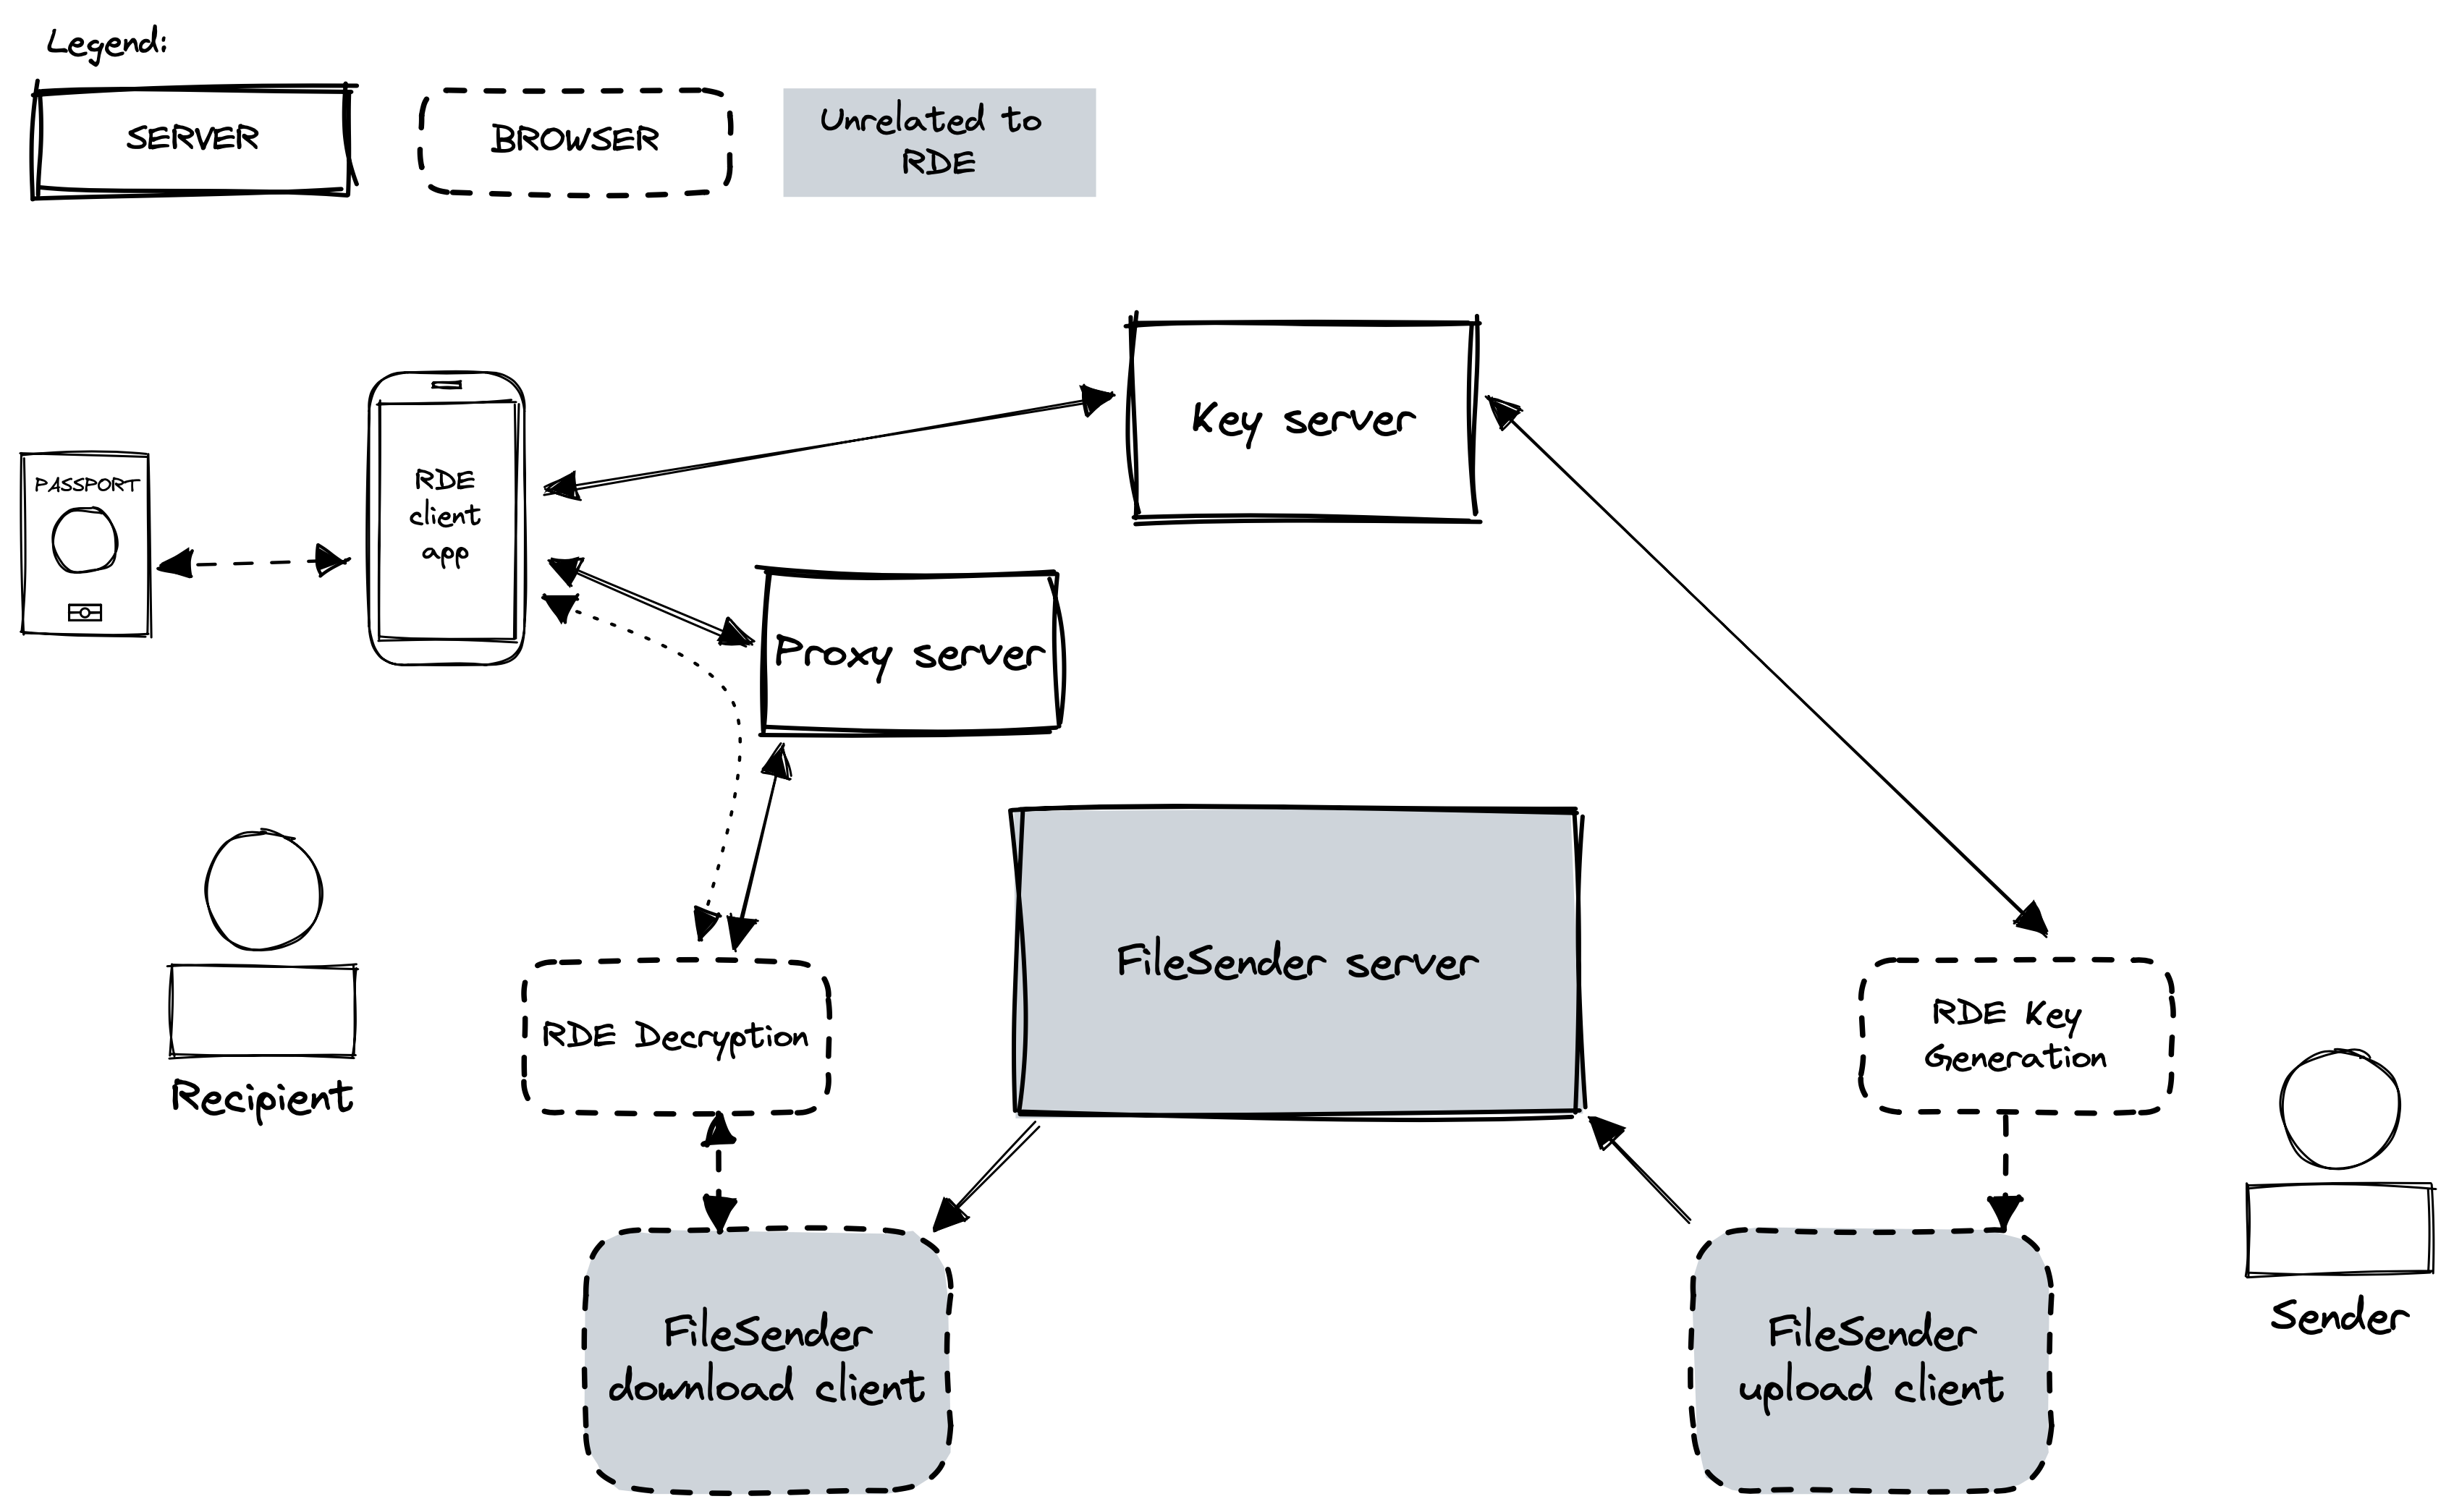
\includegraphics[width=\linewidth]{imgs/Filesender infra overview}
    \caption{Overview of the RDE infrastructure integrated in the FileSender application.}
    \label{fig:filesender-infrastructure}
\end{figure}

\subsection{File upload}\label{subsec:file-upload}
Upon uploading a file, the user is presented with the possibility to choose between the regular FileSender encryption scheme and the RDE encryption scheme.
If the user chooses the RDE encryption scheme, the user is presented with a field to query a key server with a certain email address.
The browser queries the key server for the provided email address and retrieves the enrollment parameters.
The user is then presented this list with enrollment parameters that they can choose from.

\subsubsection{Verification of the enrollment parameters}
After the user has chosen an enrollment parameter, the browser verifies the enrollment parameters.
When the enrollment parameters do not pass the verification, the user is presented with an error message.
Otherwise, a notification is shown to the user with the validated information.
There are several possibilities:

\begin{itemize}
    \item The enrollment parameters could not be verified, because no security data was included.
    The user can still proceed, but the document holder is not authenticated in any form.
    We thus fully rely on the key server for the identity of the document holder.
    \item The enrollment parameters have been verified to be from a valid e-passport.
    The issuing country and validity of the signature are shown to the user.
    \item The enrollment parameters have been verified to be from a valid e-passport and the document holder's MRZ data is included.
    In this case, additionally, the MRZ data is shown to the user.]
    \item Additionally, the facial image of the document holder is shown to the user.
\end{itemize}

In a production system, we probably want to verify the enrollment parameters before they are shown to the user for selection.
The FileSender application could also put extra restrictions on what enrollment parameters are allowed to be used.
Wwe could only accept verified enrollment parameters, enrollment parameters with MRZ data, or only accept enrollment parameters that are valid for a certain period of time.
For example, it might be desirable to disallow senders to select enrollment parameters that expire before the end of the file transfer availability period, as to prevent the document holder from being unable to decrypt the file.
These are all topics for further consideration.

\subsubsection{File encryption}
After the user has chosen the RDE document to encrypt for and verified the enrollment parameters, the browser generates an RDE key.
The decryption parameters are send to the FileSender server and stored in its database.
The secret key is used as the password for the PBKDF2 key derivation function that is already implemented in the FileSender application (for password-based encryption).

We note that the reason for choosing to use PBKDF2 here is only for the convenience of developing this prototype.
In fact, there is no reason to use PBKDF2 here, as the RDE secret key is already a random key.

\subsection{File download}\label{subsec:file-download}
When the recipient tries to download a file that is encrypted with RDE, they are presented with a popup that asks them to scan a QR code with their reader app.
This triggers the RDE decryption handshake protocol as described in section~\ref{subsubsec:decryption-handshake-protocol}.
This results in the retrieval of the secret key, which was used to encrypt the files.
This key is then again used in the PBKDF2 key derivation function to finally decrypt the files.

Note that we only find out if the decryption was successful after the first blob of a file was decrypted.
If a user would try decryption with the wrong document, the key retrieval steps would not necessarily fail, but result in a different secret key and thus only the decryption would fail.
We will, however, only find out after the first blob of a file was decrypted.
This is also the current behavior of the FileSender application for password-based file encryption.

\subsection{Notes on our implementation}\label{subsec:notes-on-our-implementation}
The implementation of the RDE integration in the FileSender application for our prototype is very minimal.
The current FileSender code base, especially with regards to the UI and browser encryption and decryption, is not very modular.
This makes it difficult to integrate RDE in a clean way.
We know that the FileSender developers are working on a new version of the application, which will feature a new UI and hopefully a more modular code base.
We expect that the integration of RDE in the new version of the FileSender application will be much easier and cleaner given the modularity of the RDE components that we developed.

\subsubsection{FileSender CLI}
We also note that the FileSender application provides a CLI tool.
We have not implemented RDE for this CLI tool, as this has not been a priority for us.

\subsubsection{The recipient}
The current FileSender integration does not enforce that the download link of the transfer is only shared with the email address that is associated with the enrollment parameters.
For a production system, this probably should be enforced for usability reasons.

\subsubsection{User interface}
In line with the rest of our prototype, the user interface of the RDE integration in the FileSender application should be improved so users better understand what is going on and users do not make unfair assumptions about the security of the system.

